\newpage
\section{Robust Principal Component Analysis}
Goal: Find a low rank representation of a matrix $X$, which is corrupted by a sparse perturbation or sparse structured noise.
\begin{figure}[H]
\centering
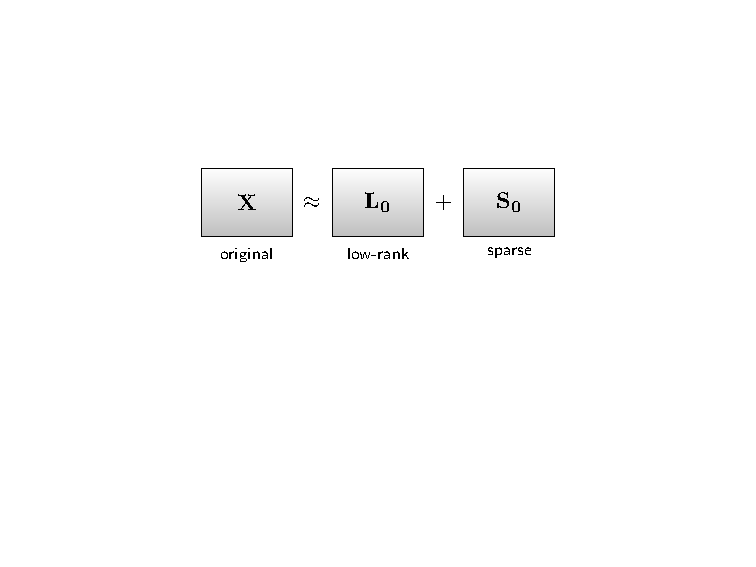
\includegraphics[width=.8\textwidth]{img/11_rpca}
\end{figure}
In contrast to the topic we have discussed so far we have compute a \emph{additive decomposition}.

\subsection{Additive Decomposition Problem}
\begin{align*}
     \text{minimise}\ &rank(L)+\lambda\cdot card(S)\\
     \text{subject to}\ &L+S =X,
\end{align*}
where $card(\cdot)$ counts the number of non-zero entries.

This optimisation problem formalises the notion of separating a matrix into a low-rank and a sparse one. However, this decomposition is difficult to compute in general. For instance, it is not a convex optimisation problem.

\subsection{Principal Component Pursuit (PCP)}
\begin{align*}
     \text{minimise}\ &\norm{L}_* +\lambda \norm{S}_1,
     \text{subject to}\ &L+S =X,
\end{align*}
where $\norm{\cdot}$ denotes the nuclear norm:
\begin{align*}
    \sum_{i=1}^{\min\{m,n\}} \sigma_i,
\end{align*}
where $\sigma_i$ denotes the $i$'th singular value of a $n\times m$ matrix and $\norm{\cdot}_1$ denotes the sum of absolute values of all matrix entries.

Note that this is not the same problem as minimising $rank(L) + \lambda\cdot card(S)$. The $L1$-Norm is only a convex relaxation of cardinality and the nuclear norm a convex relaxation of the rank.


But this relaxation will allow us to efficiently solve the problem, and if we are fortunate (i.e. under some conditions on the sparsity and low-rankness of our matrices) we recover the original matrices. We will see that this coincidence of solutions happens under surprisingly broad conditions.


In contrast to the additive decomposition problem, \emph{PCP} is \emph{convex}.

\subsection{Lagrange Mutlipliers} $\ $
\subsubsection{Primal Optimisation Problem}
\begin{align*}
    \text{minimise}\ &f(x)\\
    \text{subject to}\ &g_i(x)\leq 0&i\in[1,m]\\
     &h_i(x) =0 &i\in[1,p]
\end{align*}
\subsubsection{Unconstrained Problem} $\ $
\begin{align*}
    \text{minimise}\ &f(x) + \sum_{i=1}^m I_- (g_i(x)) + \sum_{i=1}^p I_0(h_i(x))\\
        I_-(u) &= \begin{cases}
                     0 &u\leq 0\\
                     \infty &u>0
                 \end{cases}\\
        I_0(u) &=
            \begin{cases}
                0 & u=0\\
                \infty &u\neq 0
            \end{cases}
\end{align*}
$I_0$ and $I_-$ penalise perturbations with violating constraints by "brick wall" penalty functions.

We can approximate $I_-(u)$ linearly with $\lambda_i u, \lambda_i \geq 0$ and $I_0(u)$ with $\nu_i u$:

\begin{align*}
    I_-(u) &\approx \lambda_i u &\lambda_i \geq 0\\
    I_0(u) &\approx \nu_i u,
\end{align*}
where $\lambda_i$ and $\nu_i$ are called Lagrange multipliers.

\paragraph{Lagrangian} \
\begin{align*}
    L(x,\lambda, \nu) =  f(x) + \sum_{i=1}^m \lambda_i g_i(x) + \sum_{i=1}^p \nu_i h_i(x).
\end{align*}
\paragraph{Lagrange dual function} \
\begin{align*}
    d(\lambda, \nu) = \inf_x L(x,\lambda, \nu).
\end{align*}

Since $\lambda_i u\leq I_-(u)$ and $\nu_i u\leq I_0 (u)$ for all $u$: The dual function is a lower bound on the optimal value of the primal problem $p^*$.
\begin{figure}[H]
    \centering
    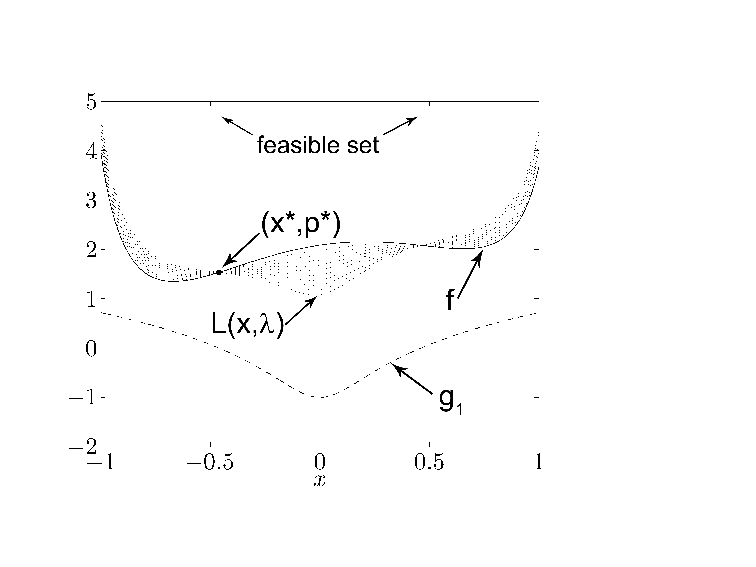
\includegraphics[width=0.7\textwidth]{img/11_lagrangian_dual_function_lower_bound}
\end{figure}

\subsection{Dual Problem}
\begin{description}
    \item[Lagrangian] \
        \begin{align*}
                L(x,\lambda, \nu) =  f(x) + \sum_{i=1}^m \lambda_i g_i(x) + \sum_{i=1}^p \nu_i h_i(x).
        \end{align*}
    \item[Lagrangian Dual Function] \
        \begin{align*}
            d(\lambda, \nu) = \inf_x L(x,\lambda, \nu).
        \end{align*}
        Now find the best lower bound on $p^*$:
    \item[Lagrange dual problem] \ 
        \begin{align*}
            \text{maximise}\ &d(\lambda, \nu)\\
            \text{subject to}\ &\lambda \geq 0
        \end{align*}
\end{description}

\emph{Strong Duality} If the primal optimisation problem is convex, under some conditions, the solution to the dual problem is equivalent to the solution of the primal problem.
It is always a lower bound on the solution of the primal problem.

In order to compute the additive decomposition for RPCA we will introduce a method called \emph{Alternating Direction Method of Multipliers}. This method builds upon two other methods, whose positive features it combines: Dual decomposition and method of multipliers.
\subsection{Convex Optimisation with Equality Constraints}
\begin{align*}
    \text{minimise}\ &f(x)\\
    \text{subject to}\ &Ax=b.
\end{align*}
\begin{description}
\item Lagrangian: $L(x,\nu) = f(x) + \nu^T (Ax-b)$
\item Dual function: $d(\nu) =\inf_x L(x,\nu)$
\item Dual problem: $\text{maximise}\ d(\nu)$
\item Recover optimal $x:\ x^*\in\argmin_x L(x,\nu^*)$ 
\end{description}

\paragraph{Gradient Method for Dual Problem}\
\begin{align*}
    \nu^{k+1} &= \nu^k +\alpha^k\nabla d(\nu^k)\\
    \nabla d(\nu^k) &= A\tilde x-b\\
    \tilde x &= \argmin_x L(x,\nu^k),
\end{align*}
\begin{itemize}
    \item $\nabla d$: Gradient of the dual function.
    \item $\alpha^k$: Step length at step $k$.
\end{itemize}

\paragraph{Dual Decomposition}
Goal: Parallelise individual optimisation steps on a cluster. 
\begin{description}
\item Suppose $f(x)$ is separable
    \begin{align*}
         f(x) &= f_1(x_1) + \ldots + f_N(x_N) &x=(x_1,\ldots, x_N)
    \end{align*}
\item Now $L$ is separable
    \begin{align*}
        L(x,\nu) &= L_1(x_1,\nu) + \ldots + L_N (x_n,\nu) - \nu^T b\\
        L_i(x_i,\nu) &= f_i(x_i) + \nu^T A_ix_i.
    \end{align*}
\item Split $x$-minimisation step and we get the dual decomposition:
    \begin{align*}
        x_i^{k+1} &:= \argmin_{x_i} L_i (x_i,\nu^k) &i\in[1,N]\\
        \nu^{k+1} &:= \nu^k + \alpha^k 
            \left(
                A_i x_i^{k+1} -b
            \right)
    \end{align*}
\item Parallelisable Algorithm:
    \begin{algorithmic}
        \STATE init $\nu^1$ and $x^1$
        \FOR{$k=2,\ldots,K$}
            \FOR{$i=1,\ldots,N$}
                \STATE // this can be parallelised
                \STATE $x_i^{k+1} :=\argmin_{x_i} L_i(x_i,\nu^k)$ $i=1,\ldots N$
                \STATE $\Theta^{k+1} = A_i x_i$
            \ENDFOR
            \STATE $\nu^{k+1} := \nu^k +\alpha^k \left(\sum_{i=i}^N \Theta^{k+1} -b\right)$ \todo{$i$ missing in $\Theta$?}
        \ENDFOR
        \STATE return $x^{k+1}$
    \end{algorithmic}
    
\end{description}

\subsection{Method of Multipliers}
To overcome some problems of Dual ascent, namely convergence only under strict convexity and finiteness of $f$ we introduce:
\paragraph{Augmented Lagrangian} \
\begin{align*}
    L_\rho (x,\nu) = f(x) + \nu^T (Ax-b)+ {\rho\over 2} \norm{Ax-b}_2^2,
\end{align*}
for any feasible $x:\ L_\rho (x,\nu) = L(x,\nu)$.
\paragraph{Method of Multipliers} \
\begin{align*}
    x^{k+1} &:= \argmin_x L_\rho(x,\nu^k)\\
    \nu^{k+1} &= \nu^k+\rho (Ax^{k+1} -b)
\end{align*}
This adds more penalty to for violating the constraints and converges under far more general conditions than dual ascent.
\subsubsection{Dual Update Step $\mathbf \rho$} Why choose $\rho$ as step size?
\paragraph{Optimality Conditions} Primal and dual feasibility
\begin{align*}
    Ax^* - b &= 0\\
    \nabla f(x^*) +A^T\nu^* &= 0.
\end{align*}
By definition $x^{k+1}$ minimises $L_\rho(x,\nu^k)$, so
\begin{align*}
    0 &= \nabla_x L_\rho (x^{k+1},\nu^k)\\
    &= \nabla_x f(x^{k+1}) +  A^T (\nu^k+\rho(Ax^{k+1} -b))\\
    &= \nabla_x f(x^{k+1}) + A^T \nu^{k+1}
\end{align*}

Therefore using $\rho$ as step size the iterate $(x^{k+1}, \nu^{k+1})$ is dual feasible. The primal residual $Ax^{k+1} -b$ converges to zero as the method of multipliers proceeds.

\subsection{Alternating Directions Method of Multipliers (ADMM)}
The main disadvantage of the method of multipliers is that the augmented Laplacian is not separable anymore. Hence we can not parallelise the $x$-minimisation step.

To get the superior convergence properties of the method of multipliers and the decomposability of dual ascent, we finally introduce the \emph{Alternating Direction Method of Multipliers} (ADMM). The method splits the variable $x$ into two parts, with the objective function separable over this splitting. The algorithm then separately minimises the two primal variables $x$ and $z$.
\begin{align*}
    \text{minimise }&f(x)+p(x) & f,\ p\text{ convex}\\
    \text{subject to }&Ax+Bz = c.
\end{align*}
\paragraph{Augmented Lagrangian} \
\begin{align*}
    L_\rho(x,z,\nu) = f(x) + p(z) +\nu^T (Ax+Bz-c) + {\rho\over 2}\norm{Ax+Bz-c}_2^2.
\end{align*}
\paragraph{ADMM}\
\begin{align*}
    x^{k+1} &:= \argmin_x L_\rho (x, z^k, \nu^k)\\
    z^{k+1} &:= \argmin_z L_\rho (x^{k+1}, z, \nu^k)\\
    \nu^{k+1} &:= \nu^k +\rho(Ax^{k+1}+Bz^{k+1}-c)
\end{align*}

\subsubsection{Optimality Conditions}
\begin{description}
\item \emph{Primal Feasibility}
    \begin{align*}
        Ax^* + Bz^* -c = 0.
    \end{align*}
\item \emph{Dual Feasibility}
    \begin{align*}
        \nabla f(x^*) +A^T \nu^* &= 0\\
        \nabla p(z^*) +B^T \nu^* &= 0
    \end{align*}
\end{description}
These primal and dual feasibility conditions are the \emph{necessary} and \emph{sufficient} optimality conditions for the ADMM problem.
It can be shown that the residual of the other two feasibility conditions converge to zero as ADMM proceeds.\\


We will show that $z^{k+1}$, one of the two primal variables, and $\nu^{k+1}$, the dual variable always satisfy the second dual feasibility condition.

\begin{align*}
    \nabla_z L_\rho (x,z,\nu) = \nabla_z p(z) + B^T \nu +\rho B^T(Ax+Bz-c)
\end{align*}
Since $z^{k+1}$ minimises $L_\rho (x^{k+1},z,\nu^k)$ by definition we have that
\begin{align*}
     0 &= \nabla_z p(z^{k+1}) + B^T \nu^k +\rho B^T (Ax^{k+1}+Bz^{k+1}-c)\\ 
     &= \nabla_z p(z^{k+1}) + B^T(\nu^k+\rho (Ax^{k+1}+Bz^{k+1}-c))\\
     &= \nabla_z p(z^{k+1}) + B^T \nu^{k+1}
\end{align*}
We observe that $z^{k+1}$ and $\nu^{k+1}$ always satisfy:
\begin{align*}
        \nabla p(z^*) +B^T \nu^* &= 0
\end{align*}

\subsection{Robustness}
\subsubsection{Classical PCA}
Classical PCA is very sensitive to outliers. \emph{One single} grossly corrupted point completely changes the principal components.
\begin{figure}[H]
    \centering
    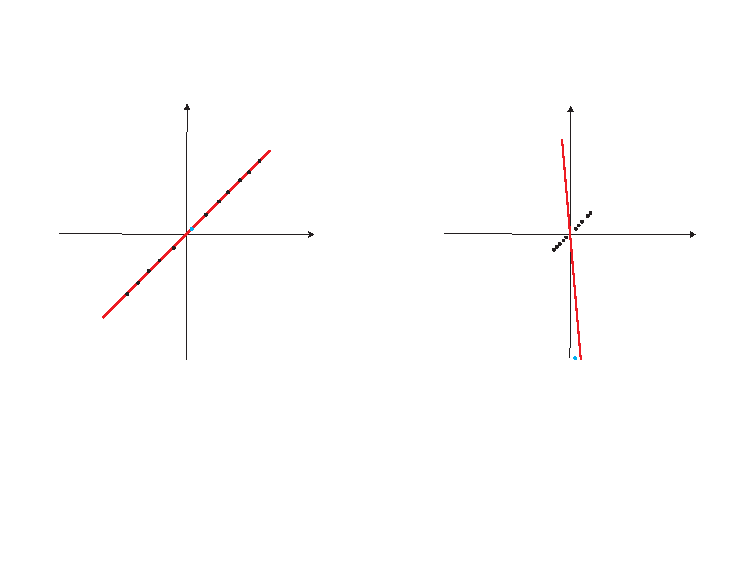
\includegraphics[width=0.7\textwidth]{img/12_pca_robustness}
\end{figure}

The main reason is that the sum of squares is minimised:
\begin{align*}
    {1\over N} \sum_{n=1}^N \norm{x_n-\tilde x_n}_2^2.
\end{align*}

\subsection{Robust PCA}
RPCA explicitly models the errors as sparse noise due to separation into low-rank and sparse matrices:
\begin{align*}
\text{minimise}\ &rank(L) + \lambda \cdot card(S)\\
\text{subject to}\ &L+S=X
\end{align*}
which can be modelled by the principal component pursuit.
\begin{align*}
    \text{minimise}\ &\norm{L}_* + \lambda \norm{S}_1\\
    \text{subject to}\ &L+S=X,
\end{align*}
where $\norm{\cdot}_*$ denotes the nuclear norm and $\norm{\cdot}$ denotes the $L_1$-norm of $S$ seen as a vector.

\paragraph{Advantages} RPCA is robust to grossly corrupted observations of $X$. It does not need to know the sparsity pattern of $S_0$. Can be easily extended to matrix completion.

\paragraph{Applications where large errors frequently occur} are
\begin{description}
    \item \emph{Image processing}: Salt \& Pepper noise
    \item \emph{Web data analysis}: Adversarial information
    \item \emph{Bioinformatics}: Spurious errors in measurements and sensor failures.
    \item \emph{Computer Vision}: Occlusions
\end{description}

\subsubsection{Recovery of $L_0$ and $S_0$}
Find the decomposition of $X$ into low rank and sparse matrix $X=L_0+S_0$:


Principal Component Pursuit (PCP):
\begin{align*}
    \text{minimise}\ &\norm{L}_* + \lambda \norm{S}_1\\
    \text{subject to}\ &L+S=X,
\end{align*}
Under broad conditions the recovery is perfect, i.e. the solution $(L^*, S^*)$ obeys:
\begin{align*}
    L^*  &= L_0,
    S^*  &= S_0.
\end{align*}

\begin{itemize}
    \item $X$ can not be low-rank and sparse.
    \item $L_0$ can not be sparse:
        \begin{align*}
            L_0 \in \R^{n\times n} &= U\Sigma M^T = \sum_{1\leq i\leq r} \sigma_i u_i v_i^T &r = rank(L_0)\\
            e_i &= (0,\ldots,0,1,0,\ldots,0)
        \end{align*}
    \item Coherence condition:
        \begin{align*}
            \norm{U^T e_i}^2 &\leq {\mu r\over n}\\
            \norm{M^T e_i}^2 &\leq {\mu r\over n}\\
            |UM^T|_{ij}^2 &\leq {\mu r\over n^2}
        \end{align*}
        This means, that Principal Components can not be sparse (spiky).
\end{itemize}

\subsubsection{Theorem}
For 
\begin{description}
\item $L_0$: $n \times n$, of $rank(L_0) \leq \rho_r n\mu^{-1}(\log n)^{-2}$
\item $S_0$: $n \times n$, random sparsity pattern of cardinality $n\leq \rho_s n^2$.

    $\rho_s$, $\rho_r$ are positive constraints.
\end{description}
With probability $1-\bigO{n^{-10}}$, PCP with $\lambda = {1\over \sqrt{n}}$ is exact.
The same holds for rectangular matrices with $\lambda= {1\over \sqrt{\max(n,m)}}$.

\subsection{Solving Robust PCA}
We want to solve
\begin{align*}
    \text{minimise}\ &\norm{L}_* + \lambda \norm{S}_1\\
    \text{subject to}\ &L+S=X.
\end{align*}
This can now be easily solved using ADMM:

We have chosen $f(x) = \norm{L}_*$ and $p(z) = \norm{S}_1$:
\begin{align*}
    L_\mu (L,S,N) &= \norm{L}_* +\lambda \norm{S}_1 + \langle N, (X-L-S)\rangle +{\mu\over 2} \norm{X-L-S}_F^2\\
    \text{with }\langle X,Y\rangle &\text{ being the Frobenius inner product: }\sum_i\sum_j X_{ij}Y_{ij}.
\end{align*}

\paragraph{ADMM for RPCA:} \
\begin{align*}
    L^{k+1} &:= \argmin_L L_\mu(S,L^k,N^k)\\
    S^{k+1} &:= \argmin_S L_\mu(S^{k+1}, L,N^k)\\
    N^{k+1} &:= N^k +\mu(X-L^{k+1}-S^{k+1})
\end{align*}
We observe that we can solve the minimisation over $L$ and $S$ explicitly:
\begin{align*}
    \argmin_S L_\mu (S,L,N) &=\mathcal S_{\lambda \mu^{-1}} (X-L+\mu^{-1}N)\\
    \argmin_L L_\mu (S,L,N) &=\mathcal D_{\mu^{-1}}(X-S+\mu^{-1}N)
\end{align*}
with
\begin{align*}
    \mathcal S_\tau(x) &= \text{sgn}(x)\max(|x|-\tau,0)\\
    \mathcal S_\tau(X) &: \text{Apply $\mathcal S_\tau$ to each element}\\
    \mathcal D_\tau(X) &= U\mathcal S_\tau (\Sigma) M^T\\
    text{where SVD } X &= U\Sigma M^T
\end{align*}

Combining all of the above we get an algorithm to solve robust PCA:


\begin{algorithmic}
    \STATE $S_0:= 0$
    \STATE $\nu_0 :0$
    \STATE $\mu > 0$
    \WHILE{not converged}
        \STATE $L^{k+1} := \mathcal D_{\mu^{-1}} (X-S^k + \mu^{-1} N^k)$
        \STATE $S^{k+1} := \mathcal S_{\lambda \mu^{-1}} (X-L^{k+1} +\mu^{-1} N^k)$
        \STATE $N^{k+1} := N^k +\mu(X-L^{k+1}-S^{k+1})$
    \ENDWHILE
\end{algorithmic}










 

























